\documentclass{standalone}
\usepackage{tikz}
\usetikzlibrary{shapes.multipart, arrows.meta, positioning}

\begin{document}
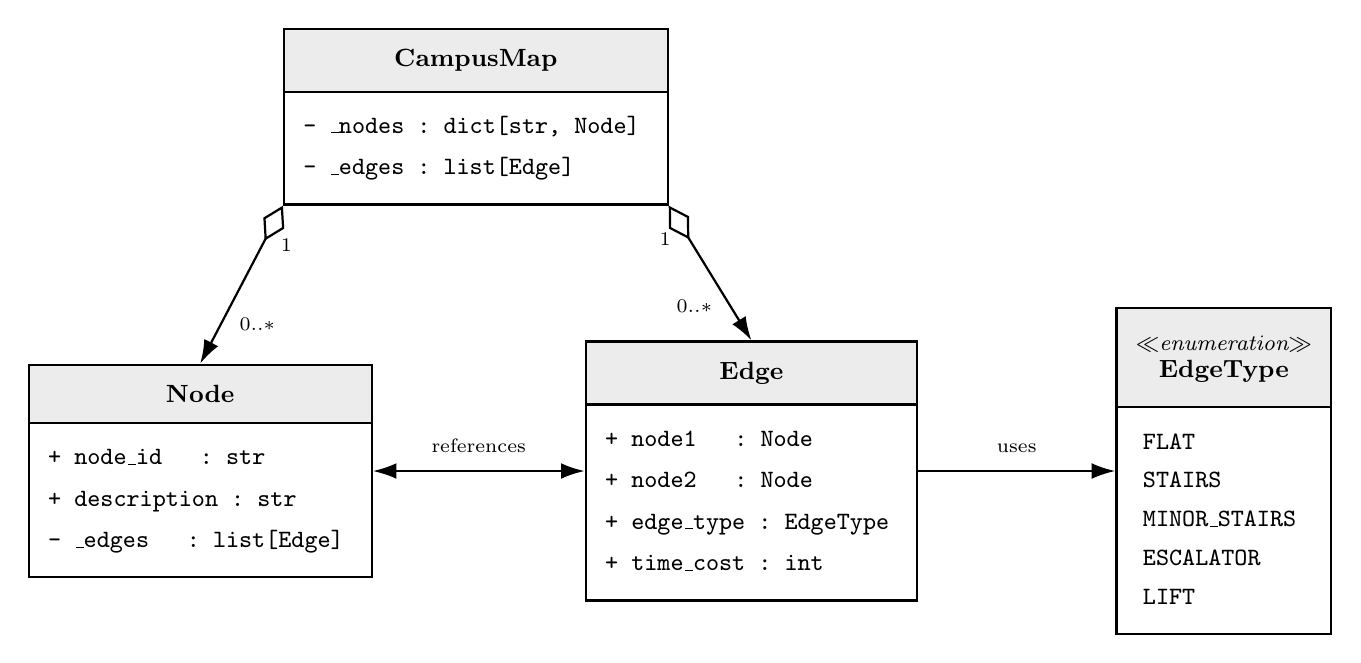
\begin{tikzpicture}[
    font=\small,
    %% ── Box styles ──────────────────────────────────────────────────────
    classnode/.style={
        draw, thick,
        rectangle split, rectangle split parts=2,
        rectangle split part fill={gray!15, white},
        inner sep=7pt,
        align=center,
    },
    enumnode/.style={
        draw, thick,
        rectangle split, rectangle split parts=2,
        rectangle split part fill={gray!15, white},
        inner sep=7pt,
        align=center,
    },
    %% ── Arrow styles ────────────────────────────────────────────────────
    %% Aggregation: open diamond at source (whole), arrowhead at target (part)
    aggr/.style={
        {Diamond[open, fill=white, length=5mm, width=3mm]}-{Latex[length=3mm, width=2mm]},
        thick,
    },
    %% Unidirectional association
    assoc/.style={
        -{Latex[length=3mm, width=2mm]},
        thick,
    },
    %% Bidirectional association
    biassoc/.style={
        {Latex[length=3mm, width=2mm]}-{Latex[length=3mm, width=2mm]},
        thick,
    },
    lbl/.style={font=\scriptsize},
]

%%─────────────────────────────────────────────────────────────────────────
%% CampusMap
%%─────────────────────────────────────────────────────────────────────────
\node[classnode] (CampusMap) at (5.5, 0) {
    \textbf{CampusMap}
    \nodepart{second}
    \begin{tabular}{@{}l@{}}
        \texttt{-\ \_nodes\ :\ dict[str,\ Node]}\\[4pt]
        \texttt{-\ \_edges\ :\ list[Edge]}
    \end{tabular}
};

%%─────────────────────────────────────────────────────────────────────────
%% Node
%%─────────────────────────────────────────────────────────────────────────
\node[classnode] (Node) at (2, -4.5) {
    \textbf{Node}
    \nodepart{second}
    \begin{tabular}{@{}l@{}}
        \texttt{+\ node\_id\quad\;\,:\ str}\\[4pt]
        \texttt{+\ description\ :\ str}\\[4pt]
        \texttt{-\ \_edges\quad\;\,:\ list[Edge]}
    \end{tabular}
};

%%─────────────────────────────────────────────────────────────────────────
%% Edge
%%─────────────────────────────────────────────────────────────────────────
\node[classnode] (Edge) at (9, -4.5) {
    \textbf{Edge}
    \nodepart{second}
    \begin{tabular}{@{}l@{}}
        \texttt{+\ node1\quad\;\,:\ Node}\\[4pt]
        \texttt{+\ node2\quad\;\,:\ Node}\\[4pt]
        \texttt{+\ edge\_type\ :\ EdgeType}\\[4pt]
        \texttt{+\ time\_cost\ :\ int}
    \end{tabular}
};

%%─────────────────────────────────────────────────────────────────────────
%% EdgeType  (enumeration)
%%─────────────────────────────────────────────────────────────────────────
\node[enumnode] (EdgeType) at (15, -4.5) {
    \begin{tabular}{@{}c@{}}
        \textit{\footnotesize$\ll$enumeration$\gg$}\\[-1pt]
        \textbf{EdgeType}
    \end{tabular}
    \nodepart{second}
    \begin{tabular}{@{}l@{}}
        \texttt{FLAT}\\[3pt]
        \texttt{STAIRS}\\[3pt]
        \texttt{MINOR\_STAIRS}\\[3pt]
        \texttt{ESCALATOR}\\[3pt]
        \texttt{LIFT}
    \end{tabular}
};

%%─────────────────────────────────────────────────────────────────────────
%% Relationships
%%─────────────────────────────────────────────────────────────────────────

%% CampusMap (1) ◇────────── (0..*) Node
\draw[aggr]
    (CampusMap.south west) -- (Node.north)
    node[lbl, near start, right=3pt] {$1$}
    node[lbl, near end,   right=3pt] {$0..*$};

%% CampusMap (1) ◇────────── (0..*) Edge
\draw[aggr]
    (CampusMap.south east) -- (Edge.north)
    node[lbl, near start, left=3pt] {$1$}
    node[lbl, near end,   left=3pt] {$0..*$};

%% Node ←──────────────────→ Edge  (bidirectional: node1/node2 and _edges)
\draw[biassoc]
    (Node.east) -- (Edge.west)
    node[lbl, midway, above=3pt] {references};

%% Edge ─────────────────────→ EdgeType  (each edge carries one EdgeType)
\draw[assoc]
    (Edge.east) -- (EdgeType.west)
    node[lbl, midway, above=3pt] {uses};

\end{tikzpicture}
\end{document}
